\section{Translational Controller} \label{sec:TranslationalController}

The translational controllers handle the movement of the quadcopter along the inertial frame directions, $x_I$, $y_I$ and $z_I$. The design structure chosen for them can be seen in \autoref{fig:TranslationalControlDiagram}.
\begin{figure}[H]
	\centering
	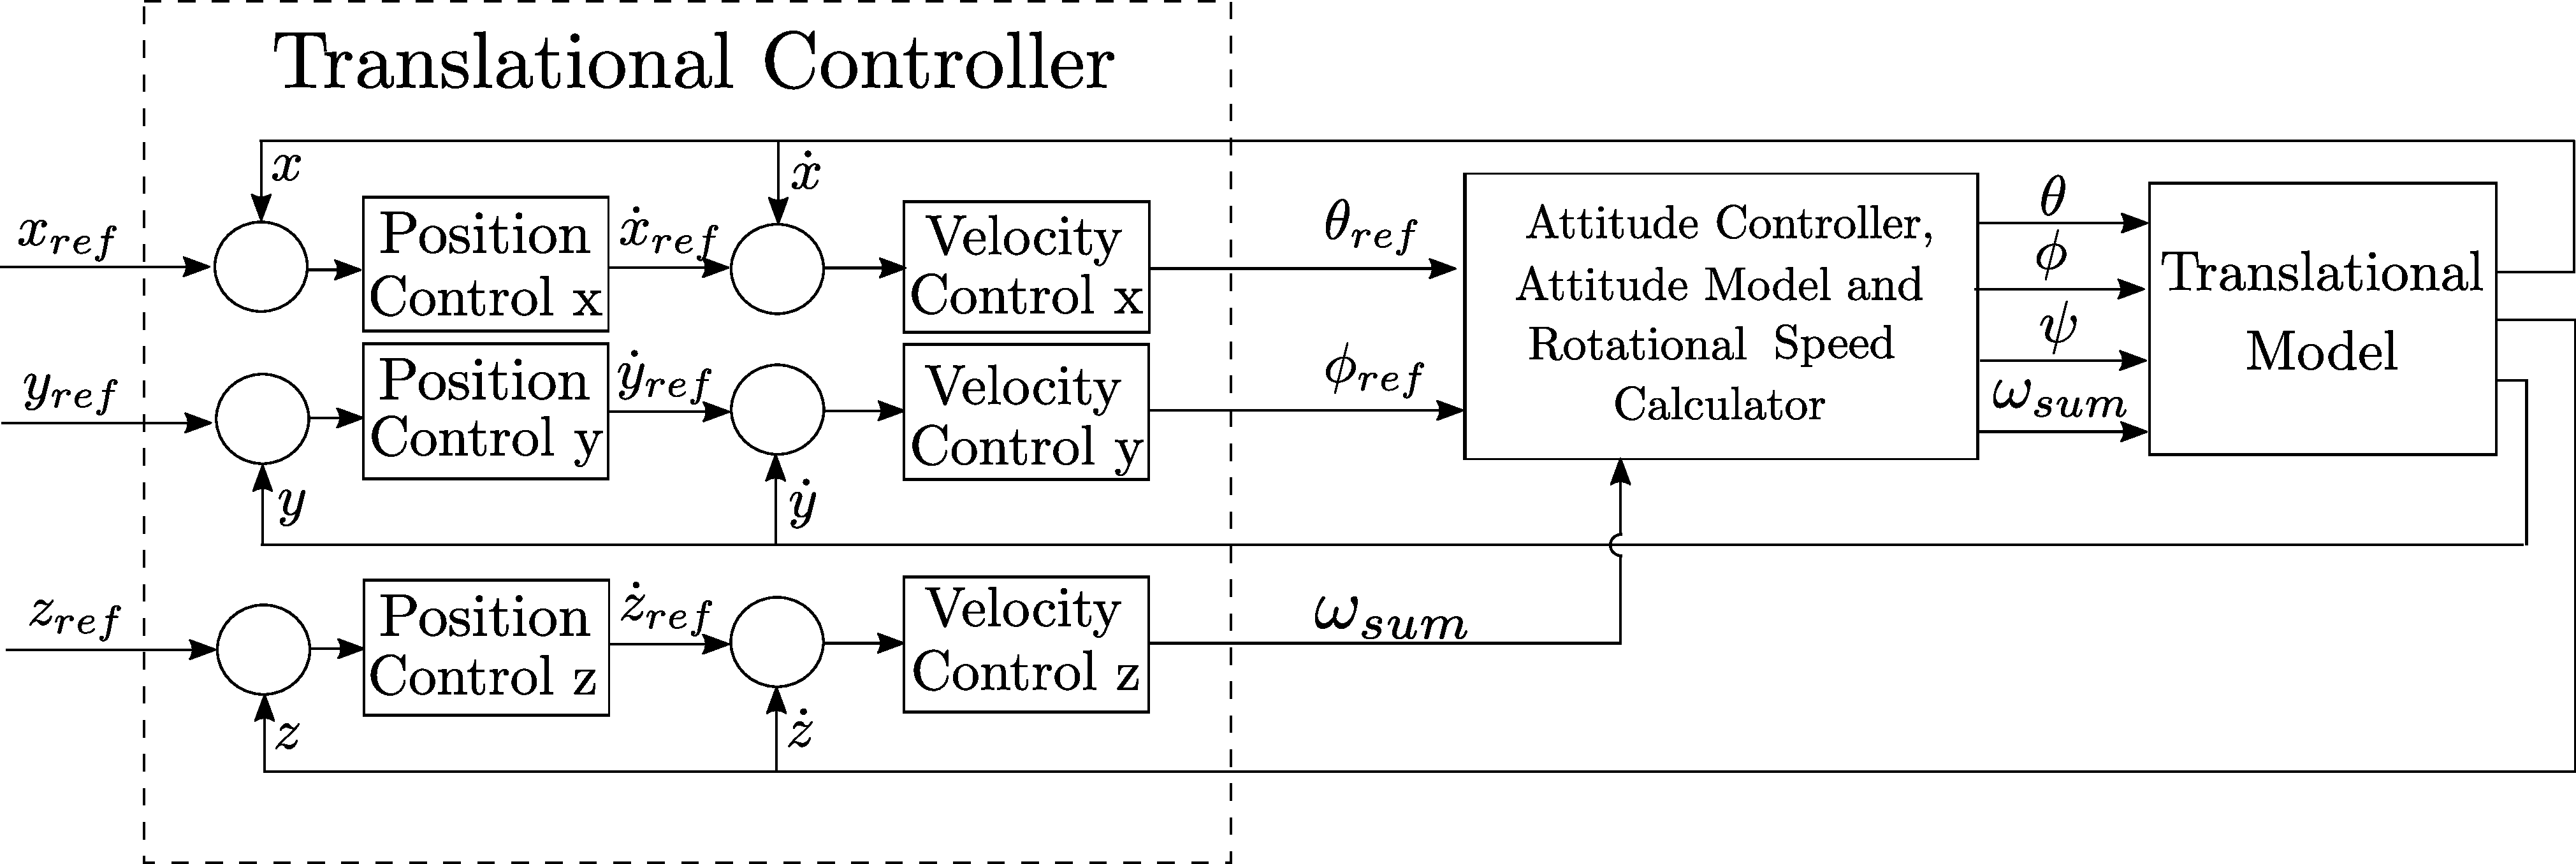
\includegraphics[scale=0.3]{figures/TranslationalControlDiagram}
	\caption{Control structure chosen for the translational controllers in the quadcopter. x and y controllers set a reference for the angular controller and the z axis controllers set the required sum of motor rotational speeds.}
	\label{fig:TranslationalControlDiagram}
\end{figure}
For each axis, the velocity and position controllers form a cascade control structure, where the position controller sets the reference for the velocity controller. In the figure it is also possible to see how x and y controllers share similar properties as both have as output an angle reference for the attitude controller, namely $\theta_{ref}$ and $\phi_{ref}$ respectively. 
The z axis position and velocity controllers set the required sum of motor rotational speeds, $\sum\omega$, such that the vertical position is attained.

In this section the design for these controllers is explained.
\subsection{Controller for z axis}
Derivation of the transfer function 

Root locus and bode

Problem with P controller (Input disturbance)

Simulation of P controller

New controller 

simulation of New controller

